
\documentclass{article}
\usepackage{amsmath,amssymb}
\usepackage[inline]{enumitem}
\usepackage{blindtext}
\usepackage{booktabs}
\usepackage{graphicx}
\usepackage{xcolor}
\usepackage[vmargin = 1.5in, top = 1in, bottom = 1.2in, letterpaper]{geometry}
\usepackage{listings}
\usepackage{courier}
\usepackage{multicol}
\usepackage{multirow}
\usepackage{bm}
\lstset{
basicstyle = \small\tt,
keywordstyle = \tt\color{blue},
commentstyle = \it\color[cmyk]{1,0,1,0},
stringstyle = \tt\color[RGB]{128,0,0},
%frame = single,
backgroundcolor = \color[RGB]{245,245,244},
breaklines,
extendedchars = false,
xleftmargin = 2em,
xrightmargin = 2em,
aboveskip = 1em,
tabsize = 4,
showspaces = false
}
\begin{document}
\setcounter{MaxMatrixCols}{20}

% \newfontfamily\courier{Courier New}


\title{STAT 510 Homework 12}
\author{Yifan Zhu}
\maketitle

\begin{enumerate}[leftmargin = 0 em, label = \arabic*., font = \bfseries]
	\item
	\begin{enumerate}
		\item 
		$\hat{\sigma}_e^2 = 3.949$
		\item 
	$\hat{\bm \Sigma}_{\bm b} = \begin{bmatrix}
		10.49 & 1.46 \times 10 ^{-3}\\
		1.46 \times 10^{-3} & 5.62 \times 10^{-5}
	\end{bmatrix}$

	\item 
	\ 
	\begin{center}
	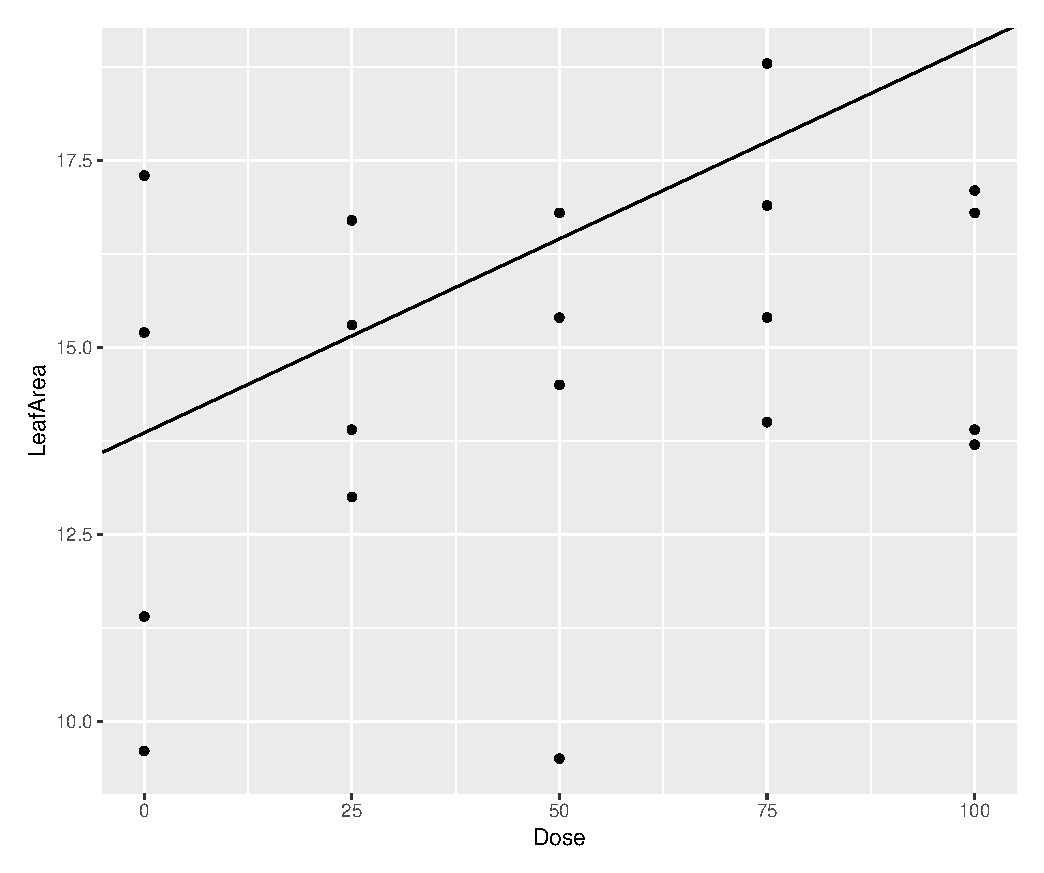
\includegraphics[width = 0.45\textwidth]{p1c.eps}
	\end{center}

	\item 
	\[12.591 + 0.044 x\]

	\item 
	\[13.650 + 0.022x\]


	\item 
	 \ 
	 \begin{center}
	 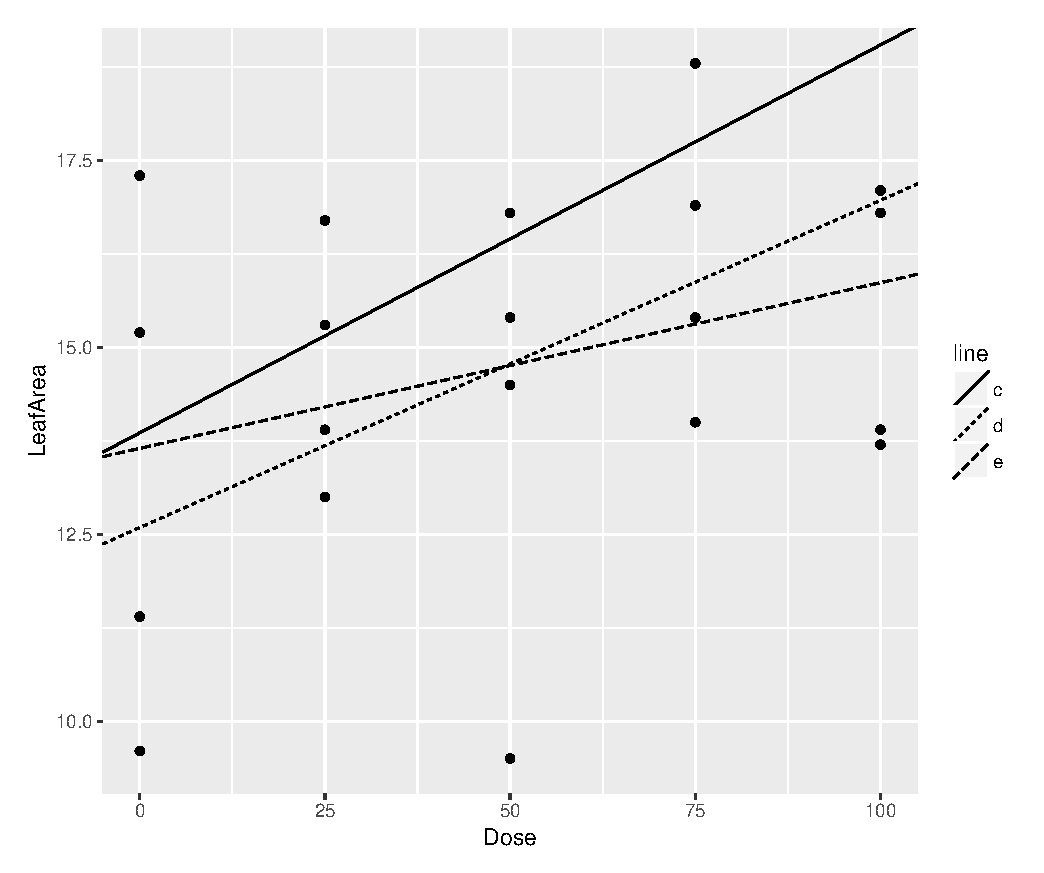
\includegraphics[width = 0.55\textwidth]{p1f.eps}
	 \end{center}


	\item 
	\[- 2 \log \Lambda = 30.73227\]

	\item 
	$AIC = 1345.905$

	\item 
	$AIC = 1342.693$

	\item 
	$AIC = 1650.107$

	\item 
	Model in part (i) is preferred. The AIC of that model is the smallest.
	
		\end{enumerate}

		\item 
		\begin{align*}
		& \bm X = \begin{bmatrix}
			\bm 1_{300}, \bm 1_{15} \otimes \begin{bmatrix}
				0 \\ 25 \\ 50 \\ 75 \ 100
			\end{bmatrix} \otimes \bm 1_{4}
		\end{bmatrix}\\
		& \bm \beta = \begin{bmatrix}
			\beta_1\\ \beta_2
		\end{bmatrix}\\
		& \bm Z = \bm I_{15 \times 15} \otimes \begin{bmatrix}
			\bm 1_{20} ,\begin{bmatrix}
				0 \\ 25 \\ 50 \\ 75 \ 100
			\end{bmatrix} \otimes \bm 1_{4} 
		\end{bmatrix}\\
		& \bm u = \begin{bmatrix}
			b_{11}\\ b_{12} \\ b_{21} \\ b_{22} \\ \vdots \\ b_{15,1} \\ b_{15 ,2}
		\end{bmatrix}\\
		& \bm G = \bm I_{15 \times 15} \otimes \bm \Sigma_{\bm b}\\
		& \bm R = \sigma_e^2 \bm I_{300 \times 300}
		\end{align*}
		\item 
		\begin{enumerate}

		\item 
		\[\bm X = \begin{bmatrix}
			\bm 1_{n_1} \otimes \bm I_{t\times t} &\\
			&\bm 1_{n_2} \otimes \bm I_{t\times t} \\
			&& \bm 1_{n_3} \otimes \bm I_{t\times t}
		\end{bmatrix}\]

		\item 
		\[\bm \Sigma = \begin{bmatrix}
			\bm I_{n_1 \times n_1} \otimes \bm W&\\
			&\bm I_{n_2  \times n_2} \otimes \bm W\\
			&& \bm I_{n_3 \times n_3} \otimes \bm W
		\end{bmatrix} = 
			\bm I_{(n_1 + n_2 + n_3) \times (n_1 + n_2 + n_3)} \otimes \bm W
		\]

		\item 
		\begin{align*}
		& \bm \Sigma^{-1} = \begin{bmatrix}
			\bm I_{n_1 \times n_1} \otimes \bm W^{-1} & \\
			& \bm I_{n_2 \times n_2} \otimes \bm W^{-1}\\
			&& \bm I_{n_3 \times n_3} \otimes \bm W^{-1}
		\end{bmatrix}\\
		& \bm X^{T} = \begin{bmatrix}
			\bm 1_{n_1}^T \otimes \bm I_{t \times t}&\\
			& \bm 1_{n_2}^T \otimes \bm I_{t\times t}\\
			&& \bm I_{n_3} \otimes \bm I_{t\times t}
		\end{bmatrix}\\
		& \bm X^{T} \bm \Sigma^{-1} = \begin{bmatrix}
			\bm 1_{n_1}^T \otimes \bm W^{-1}\\
			&\bm 1_{n_2}^T \otimes \bm W^{-1}\\
			&& \bm 1_{n_3}^T \otimes \bm W^{-1}
		\end{bmatrix}\\
		& \bm X^T \bm \Sigma^{-1} \bm X = \begin{bmatrix}
			n_1 \bm W^{-1}\\
			& n_2 \bm W^{-1}\\
			&& n_3 \bm W^{-1}
		\end{bmatrix}\\
		& (\bm X^T \bm \Sigma^{-1} \bm X)^{-1} = \begin{bmatrix}
			\frac{1}{n_1} \bm W \\
			& \frac{1}{n_2} \bm W\\
			&& \frac{1}{n_3} \bm W
		\end{bmatrix}
		\end{align*}

		\item 
		\begin{align*}
		&(\bm X^T \bm \Sigma^{-1} \bm X)^{-1} \bm X^T \bm \Sigma^{-1}\\
		 =& \begin{bmatrix}
			\frac{1}{n_1} \bm W \\
			& \frac{1}{n_2} \bm W\\
			&& \frac{1}{n_3} \bm W
		\end{bmatrix} 
		\begin{bmatrix}
			\bm 1_{n_1}^T \otimes \bm W^{-1}\\
			&\bm 1_{n_2}^T \otimes \bm W^{-1}\\
			&& \bm 1_{n_3}^T \otimes \bm W^{-1}
		\end{bmatrix} \\
		=& 
		\begin{bmatrix}
			\frac{1}{n_1} \bm 1_{n_1}^T \otimes \bm I_{t\times t}\\
			&\frac{1}{n_2} \bm 1_{n_2}^T \otimes \bm I_{t\times t}\\
			&& \frac{1}{n_3} \bm 1_{n_3}^T \otimes \bm I_{t \times t}
		\end{bmatrix}
		\end{align*}

		\item 
		\begin{align*}
		&(\bm X^T \bm \Sigma^{-1} \bm X)^{-1} \bm X^T \bm \Sigma^{-1} \bm y\\
		=& \begin{bmatrix}
			\frac{1}{n_1} \bm 1_{n_1}^T \otimes \bm I_{t\times t}\\
			&\frac{1}{n_2} \bm 1_{n_2}^T \otimes \bm I_{t\times t}\\
			&& \frac{1}{n_3} \bm 1_{n_3}^T \otimes \bm I_{t \times t}
		\end{bmatrix}  \bm y\\
		=& \begin{bmatrix}
			\frac{1}{n_1} \sum_{j = 1}^{n_1} \bm y_{1j}\\
			\frac{1}{n_2} \sum_{j= 1}^{n_2} \bm y_{2j}\\
			\frac{1}{n_3} \sum_{j= 1}^{n_3} \bm y_{3j}
		\end{bmatrix} = 	\begin{bmatrix}
				\bar{\bm y}_{1 \cdot}\\
				\bar{\bm y}_{2 \cdot}\\
				\bar{\bm y}_{3 \cdot}
			\end{bmatrix}
		\end{align*}

		\item 
		\begin{align*}
		\bm \mu_1 = \begin{bmatrix}
			\bar{y}_{1 \cdot 1}, \bar{y}_{1 \cdot 2}, \ldots, \bar{y}_{1 \cdot t}
		\end{bmatrix}^T\\
		\bm \mu_2 = \begin{bmatrix}
			\bar{y}_{2 \cdot 1}, \bar{y}_{2 \cdot 2}, \ldots, \bar{y}_{2 \cdot t}
		\end{bmatrix}^T\\
		\bm \mu_3 = \begin{bmatrix}
			\bar{y}_{3 \cdot 1}, \bar{y}_{3 \cdot 2}, \ldots, \bar{y}_{3 \cdot t}
		\end{bmatrix}^T \\
		\end{align*}

		


		
				
		
		
			\end{enumerate}
		
		
	
	     
\end{enumerate}




	      

\end{document}